\section{Uso básico Git}
    É possível obter um repositório Git de duas formas: tornando um diretório local em um repositório Git ou clonando um repositório existente.
    \subsection{Inicializando o repositório em um diretório existente}
        Para inicializar o repositório, é necessário ir até o diretório do projeto. Uma vez dentro do diretório, basta digitar:
        \begin{lstlisting}
            $ git init
        \end{lstlisting}
        Esse comando é responsável por criar um subdiretório chamado \textit{.git} que contém os arquivos essenciais para o repositório. Nenhum arquivo está sendo rastreado ainda.
        Arquivos podem ser adicionados através do comando \textit{git add}:
        \begin{lstlisting}
            $ git add .
        \end{lstlisting}
        Ao inserir \textit{.} após o comando, você está dizendo que Git deve adicionar à área de \textit{stage} todos os arquivos não rastreados. 
        Outros exemplos de uso do comando \textit{git add}:
        \begin{lstlisting}
            $ git add *.c
            $ git add my_first_file.txt
        \end{lstlisting}
        \par Ao utilizar os dois comandos acima, você está dizendo ao Git para adicionar à área de \textit{stage} todos os arquivos que tenham a extensão \textit{.c} e para adicionar o arquivo \textit{my\_first\_file.txt}, respectivamente.
        \par Para visualizar mais opções de uso do comando \textit{git add} (ou de qualquer outro comando), você pode acrescentar o argumento \textit{-h} ou \textit{--help}:
        \begin{lstlisting}
            $ git add -h
        \end{lstlisting}
        A saída para o comando acima é a descrição de uso do comando, como mostrado na figura \ref{figura:output_git_add}:
        \begin{figure}[H]
            \caption{Saída do comando \textit{git add -h}}
            \vspace{0.5cm}
            \centering
            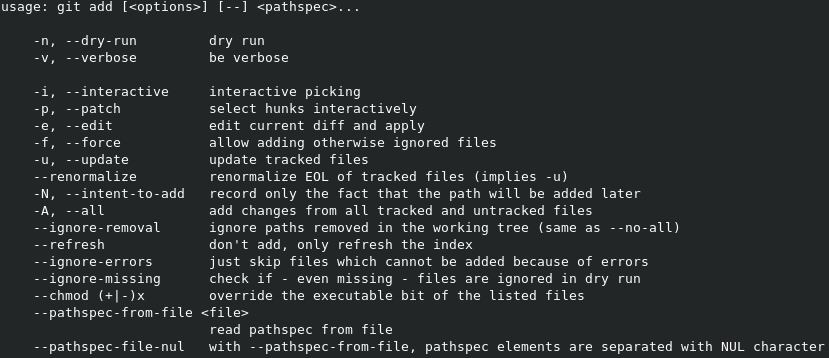
\includegraphics[width=12cm]{images/git_add_help.png}
            \label{figura:output_git_add}
        \end{figure}

        Em seguida, após selecionar os arquivos que deverão ser adicionados à área de \textit{stage}, podemos dar \textit{commit} às modificações:
        \begin{lstlisting}
            $ git commit -m "Initial project version"
        \end{lstlisting}

        Ao digitar o comando com o parâmetro \textit{-m}, você está dizendo ao Git que o commit está acompanhado da mensagem de \textit{commit} entre aspas (que pode ser simples ou dupla).
        \par É muito importante prestar atenção à maneira como você escreve a mensagem de \textit{commit}. A intenção é que ela seja assertiva, sucinta e padronizada. Normalmente, é escrita em inglês, iniciada por um verbo que indica a modificação (\textit{Add, Fix, Remove, Update, Create}) e provê uma descrição a respeito das modificações contidas no \textit{commit}.
        \par Já sabemos que um dos principais motivos para utilizar uma ferramenta de versionamento é a possibilidade de organizar e controlar eficazmente um projeto complexo e desenvolvido por várias pessoas. Nesse contexto, é de suma importância que tanto o código quanto as mensagens de \textit{commit} sejam padronizadas e, acima de tudo, sejam facilmente compreendidas por outras pessoas.
        \par Um exemplo ruim de mensagem de \textit{commit}:
        \begin{lstlisting}
            $ git commit -m "Fixed the problems with main function"
        \end{lstlisting}
        Um bom exemplo de mensagem de \textit{commit}:
        \begin{lstlisting}
            $ git commit -m "Fix seg fault on main function"
        \end{lstlisting}
        \par O objetivo é explicar qual a necessidade do \textit{commit}. Ela deve ser sucinta - você deve buscar resumir as mudanças em 50 caracteres ou menos.
        \par Também é possível dividir a mensagem de \textit{commit} em tema e corpo. Nesse caso, é possível fornecer uma explicação mais detalhada dentro do corpo, como mostrado na figura \ref{figura:mensagem_commit}:
        \begin{figure}[H]
            \caption{Mensagem de \textit{commit}}
            \vspace{0.5cm}
            \centering
            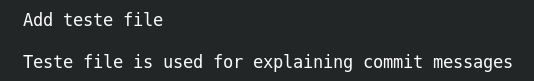
\includegraphics[width=12cm]{images/mensagem_commit.png}
            \label{figura:mensagem_commit}
        \end{figure}
        Para isso, basta inserir o comando da seguinte forma:
        \begin{lstlisting}
            $ git commit -m "Add teste file" -m "Teste file is used for explaining commit messages"
        \end{lstlisting}

        Às vezes, você quer salvar o progresso em um projeto dentro de um commit para poder fazer upload no Github e deixar as modificações seguras, caso algo dê errado com seu computador ou com sua cópia local. No entanto, você não quer que os outros contribuidores vejam o novo \textit{commit} e pensem que a tarefa está terminada. Uma boa prática é adicionar a \textit{tag} '[WIP]' - \textit{Work in Progress} - no início do \textit{commit}, como ilustrado na figura \ref{figura:exemplo_tag}:
        \begin{figure}[H]
            \caption{\textit{Commit} com trabalho não finalizado}
            \vspace{0.5cm}
            \centering
            
\includegraphics[width=12cm]{images/exemplo_tag.png}
            \label{figura:exemplo_tag}
        \end{figure}
